\documentclass[11pt, oneside]{article} 
\usepackage{geometry}
\geometry{letterpaper} 
\usepackage{graphicx}
	
\usepackage{amssymb}
\usepackage{amsmath}
\usepackage{parskip}
\usepackage{color}
\usepackage{hyperref}

\graphicspath{{/Users/telliott//Github/precalculus/fig/}}
% \begin{center} \includegraphics [scale=0.4] {gauss3.png} \end{center}

\title{Volume of a pyramid}
\date{}

\begin{document}
\maketitle
\Large

We need a formula for the volume of a cone in order to find the volume of the sphere.  And in order to find the cone's volume, we start with something simpler, a pyramid with a square base.  

Consider a cube with all eight edges having length $s$.  So each of the six faces is a square with sides of length $s$ and area $s^2$.

Label the central point inside the solid as $P$.  Draw lines connecting each of the 8 external vertices to $P$, something like this. 
\begin{center}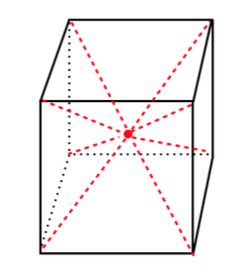
\includegraphics [scale=0.5] {cube_to_cone.png}\end{center}

Now we imagine slicing on planes that connect adjacent pairs of lines.  

You can't do this in real life by slicing up a single cube or rectangular solid, because the cuts to form one surface would ruin some of the other pieces.  The cuts must enter the solid at a corner and then pivot on a line ending at the exact center.

Perhaps you could do it with a \emph{light saber} since the beam comes to a point.

\begin{center}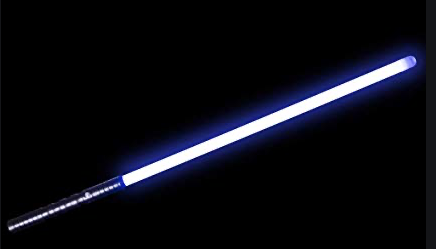
\includegraphics [scale=0.4] {light_saber.png}\end{center}

The result would be 6 identical pieces (square pyramids) looking something like this
\begin{center}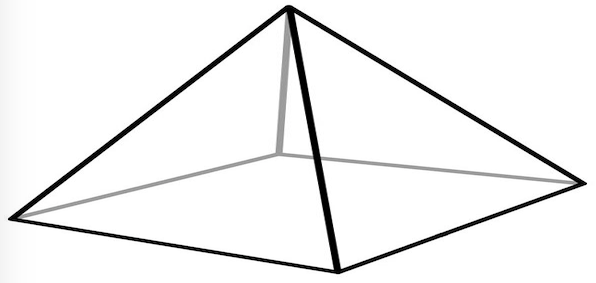
\includegraphics [scale=0.2] {sq_pyramid.png}\end{center}

The procedure described generates pyramids with height $s/2$.  So they are a little squat, but just bear with me.

We started with a cube so that the six resulting solids would be identical.  

Unfortunately you can either have six pieces come out exactly the same, as we've done, or make it so some of the pieces come out with equal base and height, but you can't do both at the same time by this construction.

Let the six identical pyramid volumes each be $V$, and their sum is equal to the volume that we started with.  We have that
\[ 6V = s^3 \]
\[ V = \frac{1}{6} s^3  \]

If we factor out the height $h = s/2$ we obtain
\[ V = \frac{1}{3} \ hs^2 \]

This is the volume for each pyramid with base area $s^2$ and height $s/2$.  

The volume depends on both the area of the base and the height.  You can show this by starting with solids that are longer in one-dimension.  Since here $h = s/2$ it all works out.

\subsection*{better way}

Here is an even better way to slice a cube

\begin{center}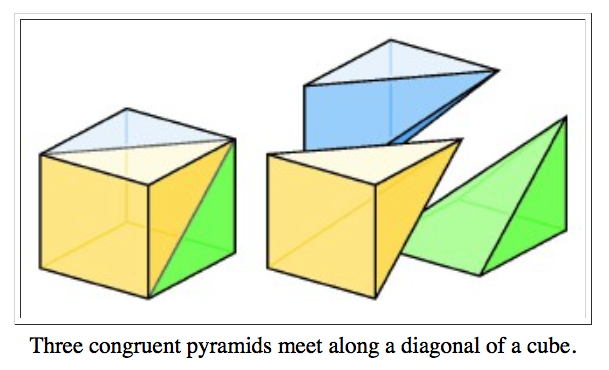
\includegraphics [scale=0.5] {pyramid_cube.png}\end{center}

When I first saw this, I thought it was a trick.  But in fact, we have produced $3$ identical pyramids (they are called oblique because the apex is not in the center).

\url{http://www.math.brown.edu/~banchoff/Beyond3d/chapter2/section02.html}

I know it sounds complicated but it's really not.

\subsection*{real world}

I found a fun way to do the demonstration easily and safely.  I was going to cut some wood on the table saw, but this is way better.

Get a thick piece of cheese and cut out a cube as large as you can make it and with everything squared up as accurately as you can.

Then cut straight down on a diagonal all the way through the cube, resulting in two identical pieces.

If you now take each of the pieces and orient them with the new angled surface resulting from the cut facing up, you can then make another diagonal cut straight down for each.  

\begin{center}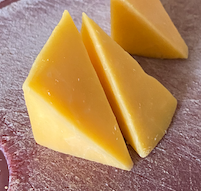
\includegraphics [scale=0.75] {cheese2.png}\end{center}

You will end up with a large piece and a small one.  Do the same with the other half.

It seems remarkable, but the two smaller ones can be assembled into a single shape identical to each of the large pieces.  

\begin{center}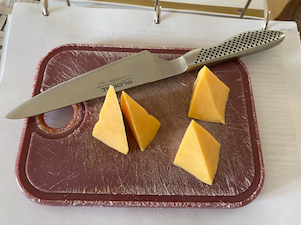
\includegraphics [scale=1.0] {cheese1.png}\end{center}

You have thus de-constructed the cube into three identical pyramids.

Good luck!  It is OK to eat the demonstration afterwards.

\subsection*{cones}

Of course, a pyramid is not a cone.  But it will turn out that the volume is independent of the shape of the base.  It just depends on the area.  This is proved by what seem to be hand-waving arguments before calculus.

For example, there is Cavalieri's principle, also called the \emph{method of indivisibles}, or the stack of quarters argument.
\begin{center}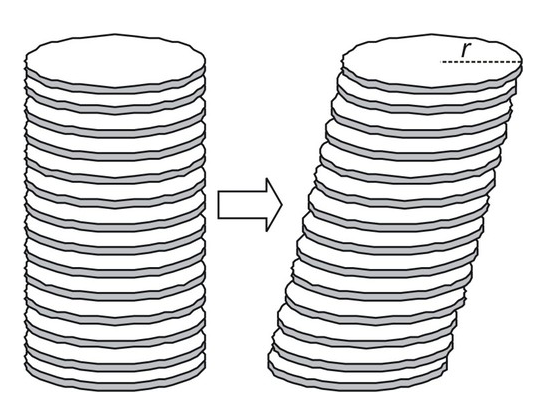
\includegraphics [scale=0.2] {volume_cone_quarters.png}\end{center}

If we slice a volume into small segments and then slide the slices around, the volume doesn't change.  So we expect that a pyramid and a right pyramid of the same base and height have the same volume, and this is in fact true.

\url{https://en.wikipedia.org/wiki/Cavalieri's_principle}

\begin{center}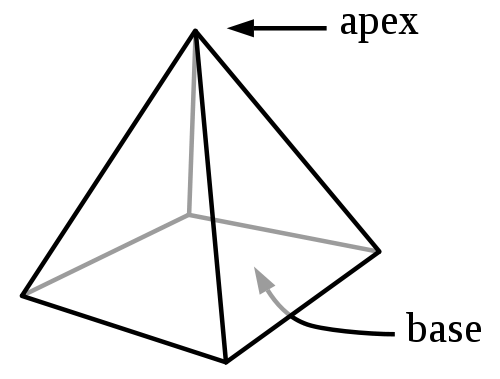
\includegraphics [scale=0.25] {volume_cone_rtpyr.png}\end{center}

And there doesn't seem any reason why the shape of the base should matter either, only its area.  Hence we substitute a circular cross-section, i.e., a cone.

For a cone we finally obtain
\[ V =  \frac{1}{3} \pi r^2 h \]

Knowing basic calculus allows us to see easily where the factor of one-third comes from in the formula for the volume of a pyramid or a cone.  It comes from integrating $x^2 \ dx$ and obtaining $x^3/3$.  Get there we will, young padawan.

However, it is interesting to see how things might have been glimpsed in the age before calculus.

\subsection*{algebraic derivation of the constant 1/3}

I found an algebraic argument on the web at 

\url{https://web.maths.unsw.edu.au/~mikeh/webpapers/paper47.pdf}

Let us assume for this proof that the volume of a cone is proportional to both the area of the base and the height:  $V = cAh$;  our objective is to find the constant of proportionality.

It takes a bit of algebra to see, but gives the value for the proportionality constant as $1/3$.

Consider a conical frustum, a cone with the top lopped off.  

\begin{center} 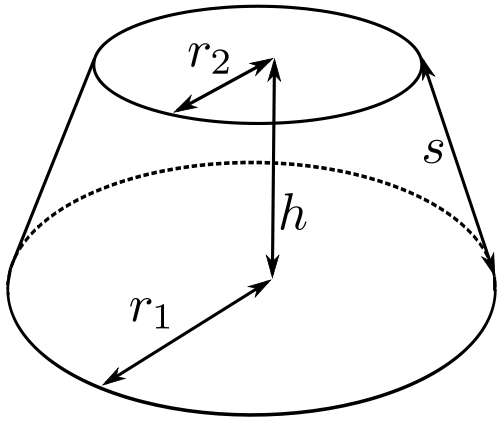
\includegraphics [scale=0.3] {conical_frustum.png} \end{center}

Suppose the area of the base is $A$ and the height of the frustum is $h$.  

Calculate the volume of the frustum as the difference between that of a larger cone with base $A$ and height $h + e$ (e for extra), and that of a small cone (the part cut off to form the frustum) with base area $a$ and height $e$.

\[ V = cA(e + h) - cae \]

Now, the area of the base of a cone is $\pi$ times the radius squared, and the radius is proportional to the height (depending on how sharply the side slants).  Hence
\[ a = \pi r_2^2 = ke^2 \]

The area of the small base is proportional to the height squared, and so is the large one, with the same proportionality constant:
\[ A = k(e + h)^2 \]
thus
\[ \frac{a}{A} = \frac{ke^2}{k(e + h)^2} \]
\[ \frac{\sqrt{a}}{\sqrt{A}} = \frac{e}{e + h} \]

Let us manipulate this expression to find $e$ in terms of $h$.  It just requires a bit of facility with square roots:

\[ \frac{\sqrt{A}}{\sqrt{a}} = \frac{e + h}{e} = 1 + \frac{h}{e} \]
\[ \frac{h}{e} = \frac{\sqrt{A}}{\sqrt{a}} - 1 \]
\[ = \frac{\sqrt{A} - \sqrt{a}}{\sqrt{a}} \]
\[ e = \frac{\sqrt{a}}{\sqrt{A} - \sqrt{a}} \cdot h \]

And then
\[ e + h = \ [ \  \frac{\sqrt{a}}{\sqrt{A} - \sqrt{a}} + 1 \ ] \ h =\frac{\sqrt{A}}{\sqrt{A} - \sqrt{a}} \cdot h \]

Substituting into what we had above for the volume:
\[ V = cA(e+h) - cae \]
\[ = cA \ [ \frac{\sqrt{A}}{\sqrt{A} - \sqrt{a}} \cdot h \ ] - ca \ [ \frac{\sqrt{a}}{\sqrt{A} - \sqrt{a}}  \cdot h \ ] \]
\[ = c \ [ \   \frac{A \sqrt{A} - a \sqrt{a}}{\sqrt{A} - \sqrt{a}} \ ] h \]

This really looks like a mess.  

But suppose we let $m =  \sqrt{A}$ and $n =  \sqrt{a}$ so
\[ \sqrt{A} - \sqrt{a} = m - n \]
then the numerator above is really just $m^3 - n^3$.    

We can factor that, we get 
\[ m^3 - n^3 = (m-n)(m^2 + mn + n^2) \]
which you can confirm by multiplying back out.  So the first term $(m-n)$ cancels the denominator.  We now have:

\[ V = c (m^2 + mn + n^2) h \]
\[ V = c (A + \sqrt{A} \sqrt{a} + a) h \]

Here's the point:  consider what happens as $a$ gets larger and closer to $A$.

We say:  let $a \rightarrow A$.

The expression in parentheses becomes $3A$.  Hence:
\[ V = c(3A)h \]
But if $a = A$, the frustum has become a cylinder, whose volume we know.  It is equal to $Ah$. 
\[ V = c(3A)h = Ah \]

Therefore $c = 1/3$.

$\square$

\end{document}